\newpage
\section{动态规划算法}

基于 DP 的 RL:
\begin{itemize}
    \item 策略迭代:
    \begin{itemize}
        \item 策略评估: 使用贝尔曼期望方程得到策略状态价值函数, 是个 DP 过程
        \item 策略提升
    \end{itemize}
    \item 价值迭代: 直接使用贝尔曼期望方程 DP, 得到最优状态价值. 
\end{itemize}

需要事先知道状态转移函数和奖励函数, 且仅适用于有限马尔可夫决策过程, 状态空间和动作空间是离散且有限的. 


\subsection{策略迭代算法}
策略迭代通过策略评估和策略提升不断交替直至得到最优策略.


\subsubsection{策略评估}
根据贝尔曼期望方程:
\begin{align*}
    V^\pi(s)=\sum_{a\in\AC}\pi(a|s) \left[ r(s,a) + \gamma \sum_{s'\in\SC} P(s'|s, a)V^\pi(s') \right]
\end{align*}
可以通过上一轮的价值状态计算下一轮的价值状态
\begin{align*}
    V^{k+1}(s)=\sum_{a\in\AC}\pi(a|s) \left[ r(s,a) + \gamma \sum_{s'\in\SC} P(s'|s, a)V^{k}(s') \right]
\end{align*}
选定初值 $V^0$, 且得知 $V^k=V^\pi$ 是更新公式的不动点. 或者说当 $k\to\infty$ 时, $\{ V^k \}$ 会收敛到 $V^\pi$. 以此计算策略的状态价值函数. 

在实际使用中, 因为贝尔曼期望方程计算代价过大, 所以当 $\max_{s\in\SC}| V^{k+1}(s)-V^k(s) |<\epsilon$ 时会提前结束策略评估. 

\subsubsection{策略提升}
得到策略状态价值函数后, 可以以此改进策略. 

\begin{theorem}[策略提升定理]
    假设存在一个确定性策略 $\pi'$, $\forall s\in\SC$, 有:
    \begin{align*}
        Q^\pi(s, \pi'(s))\ge V^\pi(s)
    \end{align*}
    则
    \begin{align*}
        V^{\pi'}(s)\ge V^\pi(s)
    \end{align*}
\end{theorem}

\begin{proof}
    $\pi'$ 在每个状态的价值不低于 $\pi$ 在该状态的价值.
    \begin{align*}
        V^\pi(s)&\le Q^\pi(s, \pi'(s))\\
        &= \E_{\pi'}[R_t + \gamma V^\pi(S_{t+1})|S_t=s]\\
        &\le \E_{\pi'}[R_t + \gamma Q^\pi(S_{t+1}, \pi'(S_{t+1}))|S_t=s]\\
        &\le \E_{\pi'}[R_t + \gamma R_{t+1} + \gamma^2 Q^\pi(S_{t+1}, \pi'(S_{t+1}))|S_t=s]\\
        &\vdots\\
        &\le \E_{\pi'}[R_t + \gamma R_{t+1} + \gamma^2 R_{t+2} + \dots |S_t=s]\\
        &= V^{\pi'}(s)
    \end{align*}
    每一步都用到了 $V^\pi(S_{t+1})\le Q^\pi(S_{t+1}, \pi'(S_{t+1}))$.
\end{proof}

于是直接贪心在每个状态选择动作价值最大的动作,
\begin{align*}
    \pi'(s)&=\argmax_a Q^\pi(s,a)\\
    &=\argmax_a \left\{ r(s,a) + \gamma \sum_{s'}P(s'|s,a)V^\pi(s') \right\}
\end{align*}
$\pi'$ 至少不比 $\pi$ 差, 当二者相同时, 则得到最优策略. 

\subsubsection{收敛性证明}

在有限马尔可夫决策过程中, $\gamma<1$, 存在上界 $C=\frac{R_{max}}{1-\gamma}$, 对于 $\forall \pi, s$, 有 $V^\pi(s)<C$. 对于每个 $s$, 其策略迭代得到的价值组成数列 $\{ V^{\pi^k} \}_{k=1,\dots,\infty}$, 根据实数单调有界收敛定理, 该数列一定收敛, 所以策略迭代算法一定收敛. 


\subsection{价值迭代算法}
价值迭代可以看做是一种只进行一轮策略评估的策略迭代算法. 价值迭代中不存在显示策略, 只维护一个状态价值函数. 

其利用贝尔曼最优方程:
\begin{align*}
    V^*(s)&=\max_{a\in\AC}\left\{ r(s,a) + \gamma \sum_{s'\in\SC} P(s'|s,a) V^*(s') \right\}
\end{align*}
改写为迭代形式:
\begin{align*}
    V^{k+1}(s)&=\max_{a\in\AC}\left\{ r(s,a) + \gamma \sum_{s'\in\SC} P(s'|s,a) V^k(s') \right\}
\end{align*}
当 $V^{k+1}=V^k$ 时, 其为贝尔曼方程不动点, 此时是最优状态价值函数, 然后利用
\begin{align*}
    \pi(s)=\argmax_a\left\{ r(s,a) + \gamma \sum_{s'\in\SC}P(s'|s,a)V^{k+1}(s')  \right\}
\end{align*}
计算出最优策略.

\subsubsection{收敛性证明}
将迭代更新的公式定义为一个贝尔曼最优算子 $\TC$:
\begin{align*}
    V^{k+1}(s)&=\max_{a\in\AC}\left\{ r(s,a) + \gamma \sum_{s'\in\SC} P(s'|s,a) V^k(s') \right\}\\
    &=\TC V^k(s)
\end{align*}

\begin{definition}[压缩算子]
    若 $\OC$ 是一个算子, 如果满足 
    \begin{align*}
        \norm{\OC V-\OC V'}_q\le \norm{V-V'}
    \end{align*}
    则称 $\OC$ 为压缩算子. 其中 $\norm{x}_q$ 表示 $x$ 的 $L_q$ 范数.
\end{definition}
这里用到无穷范数 $\norm{x}_\infty = \max_i |x_i|$

当 $\gamma <1 $ 时, 贝尔曼最优算子 $\TC$ 是一个 $\gamma-$压缩算子:
\begin{align*}
    \norm{\TC V-\TC V'}_\infty =& \max_{s\in \SC} \left| \max_{a\in\AC} \left\{ r(s,a) + \gamma \sum_{s'\in\SC} P(s'|s,a) V(s') \right\} \right. \\
    & -  \left. \max_{a'\in\AC} \left\{ r(s,a') + \gamma \sum_{s'\in\SC} P(s'|s,a') V'(s') \right\} \right| \\
    \le & \max_{s,a}\left| r(s, a) + \gamma \sum_{s'\in\SC} P(s'|s,a) V(s') \right.\\
    &\left. - r(s,a) - \gamma \sum_{s'\in\SC} P(s'|s,a') V'(s') \right|\\
    =& \gamma \max_{s,a}\left|  \sum_{s'\in\SC} P(s'|s,a)[V(s')- V'(s')] \right| \\
    \le & \gamma \max_{s,a} \sum_{s'\in\SC} P(s'|s,a)\left| V(s')- V'(s') \right| \\
    =& \gamma \norm{V - V'}_\infty
\end{align*}

将 $V'$ 设为最优价值函数 $V^*$, 于是有:
\begin{align*}
    \norm{V^{k+1}-V^*}_\infty&=\norm{\TC V^k - \TC V^*}_\infty \\
    &\le \gamma \norm{V^k - V^*}_\infty \\
    &\vdots \\
    &\le \gamma^{k+1}\norm{V^0 - V^*}_\infty
\end{align*}

所以有 $\lim_{k\to\infty} V^k = V^*$

\subsection{环境}

\subsubsection{悬崖漫步环境}
悬崖漫步环境要求智能体从起点出发, 避开悬崖, 最终到达目标位置. 智能体每个状态有四种动作: 上下左右. 如果采取动作后触碰到边界状态不改变. 掉入悬崖或者达到目标都会结束. 每走一步奖励 -1, 掉入悬崖奖励 -100.

% \begin{figure}[!htb]
%     \centering
%     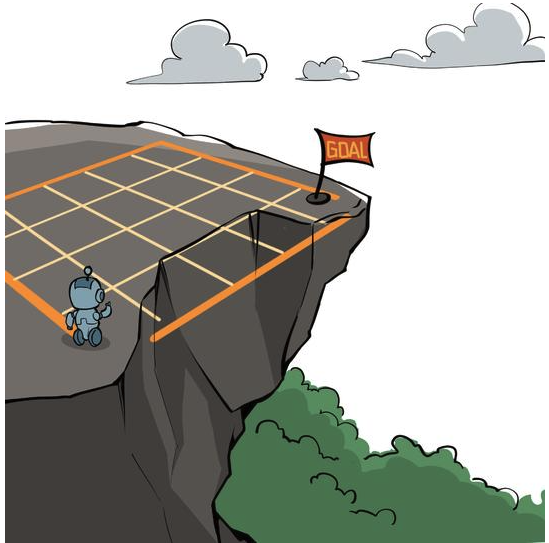
\includegraphics[width=0.618\linewidth]{pic/RL4/悬崖漫步.png}
%     \caption{悬崖漫步}
% \end{figure}

\subsubsection{冰壶环境}
引入冰洞, 进入会提前结束. 且当移动时, 有一定概率滑行到附近其他状态. 行走奖励为 0, 达到目标奖励为 1.




